
%%% Local Variables:
%%% mode: latex
%%% TeX-master: t
%%% End:

\documentclass[12pt]{article}

\usepackage{booktabs}
\usepackage{framed}
\usepackage{fullpage}
\usepackage{parskip}

% Figures
\usepackage{subfig}

% Maths
\usepackage{amsmath,amssymb,amsthm}

\newtheorem{theorem}{Theorem}[section]
\newtheorem{corollary}{Corollary}[theorem]
\newtheorem{lemma}[theorem]{Lemma}

% Algorithms
\usepackage{algpseudocode,algorithm}

% TikZ
\usepackage{tikz}

\usetikzlibrary{arrows,topaths,calc,shapes,through,intersections}

\tikzstyle{vertex}=[circle,fill=black,minimum size=10pt,inner sep=0pt]
\tikzstyle{dual}=[draw,circle,minimum size=10pt,inner sep=0pt]
\tikzstyle{edge} = [draw,very thick,-]
\tikzstyle{weight} = [font=\small]

\newcount\mycount

% Other
\newcommand{\ra}[1]{\renewcommand{\arraystretch}{#1}}

\title{Single-Source Shortest Paths in Planar Graphs}
\author{Stuart Baker, \"{O}mer Cerraho\u{g}lu, Sebastian Claici}
\date{}

\begin{document}
\maketitle

\begin{abstract}
  We survey advances in single-source shortest paths algorithms on the special case of planar graphs. For the case of non-negative edge weights, we show $O(n\log \log n)$ algorithm and provide intuition for an optimal $O(n)$ algorithm. For arbitrary edge weights, we give a $O(n\log^2 n)$ algorithm and show how to modify it to achieve $O(n\log^2 n/\log \log n)$.
\end{abstract}

\section{Introduction}
\label{sec:introduction}

Finding shortest paths in graphs is one of the oldest combinatorial optimization problems. At least in the sense of path finding, there are references dating back to the late 1800's~\cite{wiener1873ueber}. The standard algorithm for single-source shortest paths on a graph with no negative edge weights is Dijkstra's algorithm~\cite{dijkstra1959note}.

While for general graphs the problem has been effectively solved decades ago, for the special case where the graph is planar has seen a number of surprising developments in recent years. We enumerate these here, and detail them in later sections.

For directed graphs where the edge weights are non-negative, the first improvement over $O(n\log n)$ came from Federickson who gave a $O(n \sqrt{\log n}$) bound~\cite{federickson1987fast}. This was improved nearly a decade later by Henzinger et al.\ to linear time~\cite{henzinger1997faster}. We remark that for general \emph{undirected} graphs with positive edge weights, there are known linear time algorithms for single-source shortest paths in the RAM model~\cite{thorup1999undirected}.

For directed graphs with arbitrary edge weights, there have been recent developments that greatly improve upon a naive $O(n^2)$ Bellman-Ford. In 2010, Klein, Mozes and Weimann gave a $O(n \log^2 n)$ algorithm~\cite{klein2010shortest}, which was improved to $O(n \log^2 n / \log \log n)$ shortly thereafter~\cite{mozes2010shortest}. Both algorithms make use of a $O(n \log n)$ multiple-source shortest paths algorithm due to Klein~\cite{klein2005multiple}.

The goal of this paper is to provide intuition into some of the recent developments in planar graph theory.

This paper is organized as follows: in section~\ref{sec:background} we provide background on the theorems we will need later on; in section~\ref{sec:graph-sep} we detail planar graph separators which are used extensively in divide-and-conquer planar graph algorithms. In sections~\ref{sec:nonn-edge-weights}~and~\ref{sec:arbitr-edge-weights} we detail faster algorithms for single-source shortest paths in graphs with non-negative, respectively arbitrary edge weights.

\section{Background}
\label{sec:background}

We assume the reader is familiar with basic graph theory. Planar graphs are graphs that can embedded in Euclidean space such that no two edges cross each other (a more useful characterization is given shortly). Every embedding of a planar graph delineates several faces, one of which is unbounded and represents the ``outside'' of the graph; we call this face the infinite face, and denote it by $f_{\infty}$. The following theorems are used implicitly or explicitly throughout the paper.\\

\begin{theorem}[Jordan curve theorem]
  Let $C$ be any closed curve in the plane. Removal of $C$ divides the plane into exactly two connected regions, the ``inside'' and the ``outside'' of $C$.
\end{theorem}

An interesting proof of the Jordan curve theorem that uses the non-planarity of $K_{3,3}$ was given in~\cite{thomassen1992jordan}.\\

\begin{theorem}
  Any $n$-vertex planar graph with $n \geq 3$ contains no more than $3n-6$ edges.\\
\end{theorem}

\begin{theorem}[Kuratowski's theorem]
  A graph is planar if and only if it contains neither a complete graph on five vertices, nor a complete bipartite graph on two sets of three vertices as a generalized subgraph.
\end{theorem}

An in-depth discussion of Kuratowski's theorem and a short proof are found in~\cite{thomassen1981kuratowski}. The Kuratowski subgraphs are shown in figure~\ref{fig:kuratowski}.\\

\begin{figure}[!htb]
  \centering
  \subfloat[]{
    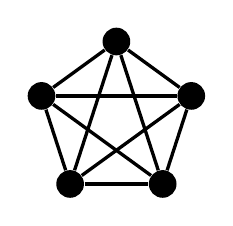
\begin{tikzpicture}[scale=0.2]
      \foreach \ang/\id in {18/1,90/2,162/3,234/4,306/5}{
        \node[vertex] (\id) at (\ang:5) {};
      }
      \foreach \number in {1,...,4}{
        \mycount=\number
        \advance\mycount by 1
        \foreach \numbera in {\the\mycount,...,5}{
          \path[edge] (\number) edge (\numbera);
        }
      }

    \end{tikzpicture}
  }\hfil
  \subfloat[]{
    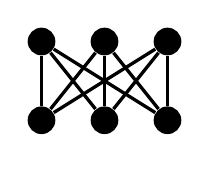
\begin{tikzpicture}[scale=0.2]
      \node at (0,-1) {};
      \foreach \x/\id in {-4/1,0/2,4/3}{
        \node[vertex] (\id) at (\x,0) {};
      }
      \foreach \x/\id in {-4/4,0/5,4/6}{
        \node[vertex] (\id) at (\x,5) {};
      }

      \foreach \x in {1,2,3}{
        \foreach \y in {4,5,6}{
          \path[edge] (\x) -- (\y);
        }
      }

    \end{tikzpicture}
  }
  \caption{Kuratowski subgraphs. (a) $K_5$, (b) $K_{3,3}$}
  \label{fig:kuratowski}
\end{figure}

\begin{theorem}
  Every planar graph can be embedded without edge crossings on a sphere. As a corollary, every node $v$ of a planar graph can be embedded on the boundary of the infinite face $f_{\infty}$.
\end{theorem}

A stereographic projection can be used to embed nodes on a plane onto a sphere without edge crossings (see figure~\ref{fig:stereo}).

\begin{figure}[!htb]
  \centering
  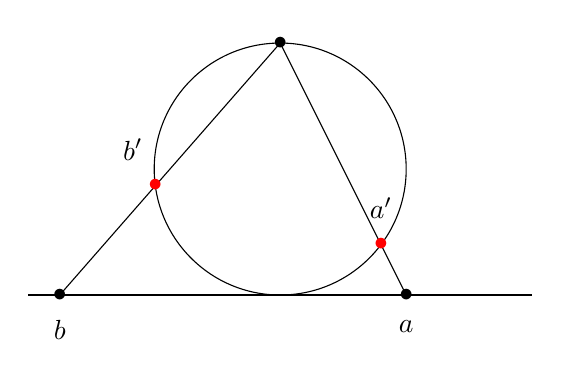
\begin{tikzpicture}[scale=0.8]
    \draw (-4,0) -- (4,0);

    \coordinate (aux) at (0,0);
    \coordinate (z) at (0,4);
    \coordinate (a) at (2,0);
    \coordinate (b) at (0,2);
    \coordinate (d) at (-3.5,0);

    \node (A) [label=270:$a$] at (a) {$\bullet$};
    \node (D) [label=270:$b$] at (d) {$\bullet$};
    \node (Z) at (z) {$\bullet$};

    \node (circ) at (b) [draw,circle through=(aux)] {};
    \coordinate (az) at (intersection 1 of circ and z--a);
    \coordinate (dz) at (intersection 1 of circ and z--d);

    \draw (a) -- (z);
    \draw (d) -- (z);

    \node (xx) [label=90:$a'$] at (az) {\color{red}$\bullet$};
    \node (yy) [label=100:$b'$] at (dz) {\color{red}$\bullet$};

  \end{tikzpicture}
  \caption{Stereographic projection of two points on a line onto a circle.}
  \label{fig:stereo}
\end{figure}

Finally, specifically for shortest paths algorithms, we use the fact that every planar graph can be transformed by adding $O(n)$ vertices and edges into another planar graph such that every node has indegree and outdegree at most $2$.

\section{Planar Graph Separators}
\label{sec:graph-sep}

    % TODO Miller's Algorithm
    % TODO Last point in Tarjan's algorithm

    \subsection{Overview}
    \label{sec:graph-sep-overview}

    For large planar graphs, a common approach to solving a specific problem is to take a divide-and-conquer approach. By dividing the problem into two or more smaller chunks and solving each subproblem, calculations that are difficult on a large scale can still be done. The core problem in divide-and-conquer problems is finding a way to divide the problem space into smaller spaces and recurse until you reach a subspace that is small enough to allow for effective computation. The results at the lowest level are then rolled back up through the recursion to give the final answer.

    In order to tackle planar graphs, there are several important relations that we rely on. If $C$ is some closed curve in the plane, by removing $C$ you can divided the plane into exactly two connected regions: the inside region and the outside region. Additionally, Kuratowski's theorem states that a graph is planar if and only if it does not have any generalized subgraphs that are either a complete graph of five nodes or a complete bipartite graph of two sets of three nodes. From Kuratowski's theorem we know that we can shrink any edge of a planar graph to a single vertex and preserve the planarity. Expanding this idea, we can shrink any subgraph of a planar graph to a single vertex and still have a planar graph.


    \subsection{Fundamental Cycle Separators}
    \label{sec:graph-sep-fund-cycle-sep}

    On method for dividing a planar graph into smaller set was developed by Lipton and Tarhan called the fundamental cycle separator~\cite{lipton1979separator}. Lipton and Tarjan showed that for any planar graph $G = (V,E)$ on $n = |V|$ vertices, and for any weight function $w: V \rightarrow \mathbb{R}^+$, it is possible to partition the nodes in the graph into three sections $A, B, C, \subseteq V$ with the following qualities.
    \begin{itemize}
        \item $w(A), w(B) \leq \alpha \cdot w(V)$ for some $\alpha \in (0,1)$

        \item There are no edges between any node in $A$ $(a \in A)$ and any other node in $B$ $(b \in B)$, $(A \times B \cap E = \emptyset)$

        \item The size of the separator $S$ is small, $|S| \leq f(n)$, specifically $\frac{2}{3}$
    \end{itemize}

    Fro a root vertex $r$, you can build a spanning tree of the graph $G$ that has depth $d$. You can then define $T^*$ as the dual tree of the triangulated version of $G$. From this tree, every non-tree edge $e$ defines a fundamental cycle $C(e)$. Since the depth of $T$ is at most $d$, we know that $|C(e)| \leq 2d + 1$. However, because the diameter of $G$ may be large, we want to reduce it so that we can constrain $|S| \leq \sqrt{n}$. Central to developing this better partition is the ability to divide the planar graph into levels. Given some $n$-vertex planar graph $G$ with nonnegative vertex costs, it is possible to partition the vertices of the graph based on their distance from a vertex $v$. One method for finding this partitioning is to run a breadth-first search from $v$. Given the partitioning, we can define $L(l)$ as the number of vertices on the level $l$ which is the distance from $v$. The levels range from $0$ to $r$ where $r$ is the maximum distance from $v$ to any vertex in the graph. For the algorithm to work, an additional, empty, level must be added at $r+1$.

    The algorithm is as follows:
    \begin{enumerate}

        \item Find the most costly component in the graph and run a depth-first search from this graph. This calculates the level of each vertex in the graph in provides the level values $(L(l))$ for every $l$. For the maximum depth $r$ in the level tree, add an additional level at $r+1$ that contains no vertices. This can be performed in $\mathcal{O}(n)$.

        \item Find the level $i_0$ that contains the median vertex. This is the level where $\sum_{i \leq i_0} |L_i(v)| \geq \frac{n}{2}$ and $\sum_{i \geq i_0} |L_i(v)| \geq \frac{n}{2}$. This can be performed in $\mathcal{O}(n)$.

        \item Find the levels $i_- \leq i_0 \leq i_+$. This can be performed in $\mathcal{O}(n)$.
        \begin{itemize}
            \item Start from the median vertex containing level $i_0$ and increase $i_+$ as well as decrease $i_-$ until $|L_{i_-}|,|L_{i_+}| \leq \sqrt{n}$

            \item Because each section can only contain half of the vertices, we can use the counting argument to state that $|i_0 - i_-|,|i_+ - i_0| \leq \frac{\sqrt{n}}{2}$

            \item At this point we have the separator $|L_{i_-} \cup L_{i_+}| \leq 2 \sqrt{n}$, which we can return if some grouping of $L_{< i_-}$, $L_{> i_+}$, and $L_{i_-,i_+}$ is balanced.
        \end{itemize}

        \item From a condensed graph $G^{'}$
        \begin{itemize}
            \item Delete or contract all edges in $L_{\geq i_+}$

            \item Contract all edges in $L_{\leq i_-}$ to form a super-vertex $v$ that is connected to all vertices $u \in L_{i_- + 1}$
        \end{itemize}


        \item From the condensed graph $G^{'}$, create a fundamental cycle separator
        \begin{itemize}
            \item Build a breadth-first tree from $G^{'}$ from $v$. This tree will have a depth $|i_+ - i_-| \leq \sqrt{n}$

            \item Triangulate the BFS tree.

            \item Apply the fundamental cycle separator lemma presented above to divide the graph into three groups.
        \end{itemize}

        \item Using this separator, return $A$ and $B$ as some combination of int$(C)$, ext$(C)$, $L_{< i_-}$, and $L_{> i_+}$. $S$ can be returned as a combination of $L_{i_-}$, $L_{i_+}$, and $C$.

        Use fundamental cycle separator and levels (step 4) to construct a satisfactory vertex partition (lemma 3). Extend the partition from the connected components chosen (step 2) to the entire graph (theorem 4).
    \end{enumerate}

    \subsection{Miller's Algorithm}
    \label{sec:graph-sep-miller}

    Miller showed an alternative method for separating a planar graph into two sections with a separator region. He showed that every 2-connected triangulated planar graph with $n$ vertices has a simple cycle $C$ of length at most $4\sqrt{n}$~\cite{miller1984finding}. Like Lipton and Tarjan's algorithm, Miller's algorithm produces two sets, $A$ and $B$, each of which with no more than $\frac{2}{3}n$ vertices. Miller's Algorithm consists of two distinct phases:
    \begin{enumerate}
      \item Find a subgraph $H$ of the parent planar graph $G$ that has a diameter of $\sqrt{n}$ and a face size of $\sqrt{n}$

      \item Find a separator contained in $H$
    \end{enumerate}

    Given that we now have the subgraph $H$ from the p[arent graph $G$, we now have to find the separator within $H$.
    \begin{theorem}
      If $G_\phi$is a 2-connected embedded planar graph with spanning tree $T$, then there exists a simple cycle weight separator of size at most $d + S$ with no face weight $> \frac{2}{3}$. Where $d$ is the diameter fo $T$, and $S$ is the maximum face size.
    \end{theorem}


    \subsection{r-Subdivision}
    \label{sec:graph-sep-rsub}

    The graph segmentation algorithms presented above can be used to recursively break a graph apart for a divide-and-conquer approach to solving problems. Specifically, the graph can be divided into $\Theta \left (\frac{n}{r} \right )$ regions, each of which have $\mathcal{O}(r)$ vertices and a total of $\mathcal{O} \left (\frac{n}{\sqrt{r}} \right )$ boundary vertices. Frederickson takes this definition a step further and defines a \textit{suitable} r-division of a planar graph as the r-division that satisfies two characteristics~\cite{federickson1987fast}:
    \begin{enumerate}
        \item Each boundary vertex is contained in at most three regions

        \item Any region that is not connected consists of connected components, all of which share boundary vertices with exactly the same set of either one or two connected regions.
    \end{enumerate}

    Starting with the initial graph $G$, all of the vertices are in the interior region. A separator algorithm can then be applied to the graph with all of the vertex weights set to $\frac{1}{n}$. This will produce three sets: $A$, $B$, and $C$. From these two sets, we can infer two regions that have the vertex sets $A_1 \subseteq A \cup C$ and $A_2 \subseteq B \cup C$. These two vertex sets will have sizes $\alpha n + \mathcal{O}\sqrt{n}$ and $(1 - \alpha) n + \mathcal{O}\sqrt{n}$ with $\frac{1}{3} \leq \alpha \leq \frac{2}{3}$. To continue the process, the separator algorithm can be recursively applied to any region that has more than $r$ vertices. The total runtime of this algorithm is $\mathcal{O} \left (n \log \left (\frac{n}{r} \right ) \right )$.

    However, to ensure that the two qualities that Miller enumerated hold, additional steps must be made. After applying the planar separator algorithm, there are three sets of vertices: $A$, $B$, and $C$. If we say that $C^{'}$ is the set of vertices in $C$ not adjacent to any vertex in $A \cup B$, the we can define $C^{''} = C - C^{'}$. Next, we need to identify the connected components $A_1, A_3, \ldots, A_q$ in $A \cup B \cup C^{'}$. Using this information, we can remove any vertex $v$ from $C^{''}$ and insert it into $A_i$ if that vertex is adjacent to a vertex in $A_i$, but not adjacent to a vertex in $A_j$ for $i \neq j$. This will ensure that a boundary vertex will be in at most three subgraphs. However, this does not ensure that there are at most $\Theta \left ( \frac{n}{r} \right )$ connected subgraphs. To ensure that there are no more than $\Theta \left ( \frac{n}{r} \right )$ connected subgraphs, we can apply a greedy approach. Sweep through the set of connected regions, join together any two neighboring regions that each have less than $\frac{r}{2}$ vertices. Furthermore, we have to ensure that all of the subregions do not possess more than$c \sqrt{r}$ boundary vertices. To solve this problem, we can run through the connected subgraphs and apply the separator technique to any subgraph that has more than $c \sqrt{r}$ boundary vertices. This does impose an additional requirement when merging small subgraphs that the number of boundary vertices in each group can be at most $\frac{c}{2} \sqrt{2}$.

    \subsubsection{Recursive Subdivision}
    \label{sec:graph-sep-rsub-recursive}

    % TODO See if this is good enough...

    Planar graphs can be recursively decomposed into smaller planar graphs. This allows the planar separators to be combined into a planar separator hierarchy which can be stored in a variety of data structures. One example is using a binary search trees to store the vertices within the planar graph in a hierarchical manner. Using this technique, it is possible to efficiently search within the planar graph.

\section{Single source shortest paths with nonnegative edge weights}
\label{sec:nonn-edge-weights}

\subsection{Simple algorithm}
\label{sec:simple-algorithm}

For a planar graph with nonnegative edge weights, Dijkstra's algorithm runs in $O(n \log n)$ as $m \leq 3n - 6$. It is possible to improve this to $O(n)$. To get there, recall that and $r$-division of a planar graph is a partition of the graph into $\Theta(n/r)$ regions of size $O(r)$ with boundary size $O(\sqrt{r})$. An $r$-division of a planar graph can be computed in linear time.

A simple $O(n\sqrt{\log n \log \log n})$ emerges quite beautifully just from the $r$-division if we set $r = \frac{\log n}{\log \log n}$. The algorithm follows a divide-and-conquer approach in which each region is processed first, followed by a clean-up phase where the results are merged.

\begin{algorithm}[!htb]
  \refstepcounter{algorithm}
  \label{alg:sssp-region}
  \begin{algorithmic}
    \ForAll {Regions $R$}
      \ForAll {Boundary nodes $v \in R$}
        \State Compute SSSP from $v$ in $R$
        \State Store $(u,v)$ distances for any two boundary nodes $u$, $v$
      \EndFor
    \EndFor
  \end{algorithmic}
\end{algorithm}

The first step is to compute the single-source shortest paths for each boundary node in each region $R$ (algorithm~\ref{alg:sssp-region}). We can now replace each region $R$ by a complete graph on $R$'s boundary nodes with shortest paths distances between any two nodes. Call this auxiliary graph $G'$. The second phase of the algorithm is to compute the SSSP from $s$ in $G'$. This gives the true shortest paths from $s$ to all the boundary nodes. Finally, we must tidy up by finding the distances from $s$ to the nodes inside each region (algorithm~\ref{alg:sssp-full}).

\begin{algorithm}[!htb]
  \refstepcounter{algorithm}
  \label{alg:sssp-full}
  \begin{algorithmic}
    \ForAll {Regions $R$}
      \ForAll {Boundary nodes $v \in R$}
        \State Set $d(v) = d_{G'}(s,v)$
        \State Compute SSSP from $v$ in $R$
      \EndFor
    \EndFor
  \end{algorithmic}
\end{algorithm}

To analyze the algorithm, we will need a few pieces of information:
\begin{itemize}
\item Total number of boundary nodes is $O(\sqrt{r})O(n/r) = O(n/\sqrt{r})$.
\item Number of nodes in $G'$ is $O(n/r)O(\sqrt{r})=O(n/\sqrt{r})$.
\item Number of edges in $G'$ is $O(n/r)O(r) = O(n)$.
\end{itemize}

Using $r=\frac{\log n}{\log \log n}$, the first phase is bounded above by
\[
  O\left(n\frac{\sqrt{\log \log n}}{\sqrt{\log n}} \log n\right)= O(n \sqrt{\log n \log \log n}),
\]
the second phase is an SSSP in a size $O(n \frac{\sqrt{\log \log n}}{\sqrt{\log n}})$ graph, and thus also $O(n \sqrt{\log n \log \log n})$, while the tidying up is a series of SSSPs in each of the regions, and has the same bound as the first phase---$O(n \sqrt{\log n \log \log n})$. The total time bound ends up $O(n \sqrt{\log n \log \log n})$.

\subsection{Recursion}
\label{sec:recursion}

The simple algorithm shown above is an improvement over Dijkstra's algorithm, but one can do better. In fact, we can achieve linear time by recursively subdividing the graph. Without loss of generality, assume the graph is directed, and that each node has at most two incoming and two outgoing edges. We call a region atomic if it contains only one edge $uv$. A nonatomic region will have as children subregions that are contained within it.

For each region $R$, we maintain a priority queue $Q(R)$ that stores the subregions of $R$ if $R$ is nonatomic, or the single arc $uv$ is $R$ is atomic. The algorithm ensures that for every region $R$, the minimum element of $Q(R)$ is the minimum label $d(v)$ over all edges $vw$ in $R$ that remain to be processed.


\begin{algorithm}
  \refstepcounter{algorithm}
  \label{alg:linear}
  \begin{algorithmic}[1]
    \State Find recursive subdivision $R(G), R(P_i), \ldots, R(uv)$
    \State Allocate queue $Q$ for each region
    \State $d(v) \gets \infty, \forall v$
    \State $d(s) \gets 0$
    \ForAll {$sv \in E(G)$}
      \State \Call{Update}{$R(sv),sv,0$}
    \EndFor
    \While {$Q(R(G)).minKey() < \infty$}
      \State \Call{Process}{$R(G)$}
    \EndWhile
  \end{algorithmic}
\end{algorithm}

The algorithm repeatedly calls two subprocedures \textsc{Process} and \textsc{Update} to process individual regions and update parent regions. Unlike Dijkstra's algorithm, the work we do in a region is only speculative. Often we cannot afford to fully process a region, and executions are stopped after a fixed number of steps.

\begin{algorithm}[!h]
  \label{alg:process}
  \begin{algorithmic}[1]
    \Procedure{Process}{}
      \If {$R$ contains only $uv$}
        \If {$d(v) > d(u) + c(u,v)$}
          \State $d(v) \gets d(u) + c(u,v)$
          \State for each outgoing edge $vw$ of $v$, call \Call{Update}{$R(vw),vw,d(v)$}
        \EndIf
        \State $Q(R).updateKey(uv,\infty)$
      \Else
        \Repeat
          \State $R' \gets Q(R).getMin()$
          \State \Call{Process}($R'$)
          \State $Q(R).updateKey(R',Q(R').minKey())$
        \Until {$Q(R).minKey()$ is infinity or if repeated $\alpha_{h(R)}$ times}
      \EndIf
    \EndProcedure
  \end{algorithmic}
\end{algorithm}


\begin{algorithm}[!h]
  \label{alg:update}
  \begin{algorithmic}[1]
    \Procedure{Update}{$R,x,k$}
      \State $Q(R).updateKey(x,k)$
      \If {$updateKey$ reduced the value of $Q(R).minKey()$}
        \State \Call{Update}{$parent(R),R,k$}
      \EndIf
    \EndProcedure
  \end{algorithmic}
\end{algorithm}

By playing around with the number of levels, number of nodes per region per level, and the $\alpha_i$, we can achieve linear time. To give an intuition, we present here a $O(n \log \log n)$ algorithm and briefly comment on how to change it to get rid of the $\log \log n$ factor.

\subsubsection{Correctness}
\label{sec:correctness}

Recall from Dijkstra's algorithm that three properties imply correctness:
\begin{enumerate}
\item Initialization: $d(s) = 0$.
\item Minimum length property: $d(v)$ is an upper bound on the $s$ to $v$ distance
\item Edges are relaxed: $d(v) \leq d(u) + c(u,v), \forall uv \in E$
\end{enumerate}

The first property is true at the start of the algorithm, and remains true throughout. The following lemma establishes the second property:\\

\begin{lemma}
  For each node $v$, $d(v)$ is an upper bound on the distance from $s$ to $v$ throughout the algorithm.
\end{lemma}

\begin{proof}
  Initially, all labels except $d(s)$ are infinity. The labels only get changed in line $4$ of \textsc{Process}, and assuming inductively that the old labels $d(v)$ and $d(u)$ are upper bounds on the distance to $u$ and $v$, it follows that the new labels will also be upper bounds.
\end{proof}

Similarly, the following three lemmas establish the third property.\\

\begin{lemma}
  If an edge $uv$ is inactive then it is relaxed.
\end{lemma}

\begin{proof}
  The lemma holds before the first call to \textsc{Process} as every node but $s$ has label infinity and outgoing edges from $s$ are active. Edges are deactivated only in line $7$ of \textsc{Process} which occurs only after the edge has been relaxed.

  Note that it is possible that an edge becomes unrelaxed after changes to the labels of its endpoints. This can occur for a call to \textsc{Update}, but line $2$ of \textsc{Update} changes the key of the edge, making it active again.
\end{proof}

\begin{lemma}
  The key of an active edge $uv$ is $d(u)$ (except during lines $3-6$ of \textsc{Process}).
\end{lemma}

\begin{proof}
  Whenever a label $d(u)$ is assigned a value $k$, \textsc{Update}$(R(uv),uv,k)$ is called for each outgoing edge $uv$, and the key of $uv$ is updated to $k$.
\end{proof}

\begin{lemma}
  \label{lemma:invariant}
  For any region $R$ that is not an ancestor of the current region, the key associated with $R$ in $Q(parent(R))$ is the minimum key of $Q(R)$.
\end{lemma}

\begin{proof}
  Whenever the minimum key of a queue $Q(R)$ is changed in line $2$ of \textsc{Update}, the recursive call in line $4$ ensures that the key associated with $R$ in the parent of $R$ is also changed.
\end{proof}

From lemma~\ref{lemma:invariant}, the following corollary follows:\\

\begin{corollary}
\label{cor:relaxed}
  For any region $R$ that is not an ancestor of the current region,

  \[
    Q(R).\text{minKey}() = \min \{ d(v) | \text{uv is a pending edge contained in R} \}
  \]
\end{corollary}

When the algorithm terminates, the minimum key of the priority queue associated with the entire graph will be infinity, and by corollary~\ref{cor:relaxed} all edges will be relaxed.

\subsubsection{Analysis}
\label{sec:analysis}

A recursive subdivision of a graph induces a hierarchy of levels. We will say that edges are at level $0$, and levels increase up to the region containing the entire graph.

We show that dividing the graph into $O(n/\log^4n)$ regions of size $O(\log^4 n)$ with boundaries of size $O(\log^2 n)$ and setting $\alpha_1 = \log n$ and $\alpha_2 = 1$ yields an $O(n \log \log n)$ single source shortest paths algorithm. Note that the division is simply an $r$-division with $r=\log^4 n$. There are $3$ levels in this division: the edges, the regions of the $r$-division, and the whole graph.

We restate the algorithm:
\begin{enumerate}
\item Select the region containing the lowest labeled node that has active outgoing edges in the region.
\item Repeat $\log n$ times: Select the lowest labeled node $v$ in the current region that has active outgoing edges in the region. Relax and deactive its outgoing edges $vw$ in that region. For each of the other endpoints $w$ of these edges, if relaxing the edge $vw$ resulted in decreasing the label of $w$, then activate the outgoing edges of $w$.
\end{enumerate}

The majority of the time is spent in invocations of \textsc{Process}. We say that an invocation of \textsc{Process} on region $R$ is \emph{truncated} if $Q(R).minKey()$ is infinity at the end of the invocation. All level $0$ invocations are truncated. The crux of the analysis relies on the following \emph{charging invariant} (the proof of which is in appendix A):

\noindent\makebox[\textwidth][c]{%
\begin{minipage}{.8\textwidth}
  For any pair $(R,v)$ of region $R$ and entry node $v$, there is an invocation $B$ of \textsc{Process} such that all invocations charging to $(R,v)$ are descendants of $B$ (or $B$ itself).
\end{minipage}}

Intuitively, the \emph{charging invariant} says that the number of charges to any pair is small, so the number of truncated invocations will be small.

 Let us first consider the number of pairs $(R,v)$ on each level to which we can charge truncated invocations to (recall that $v$ is an entry node into $R$):
\begin{itemize}
\item If $R$ has level $0$, then $R$ is charged by at most one level $0$ invocation. There are $O(n)$ pairs $(R,v)$ on level $0$, and thus $O(n)$ chargers.
\item If $R$ has level $1$, the pair is charged by at most one level $1$ invocation and at most $\alpha_1 = \log n$ level $0$ invocations. There are $O(n/\log^4n)\cdot O(\log^2 n)$ pairs on level $1$.
\item If $R$ has level $2$, then the pair is charged by at most one level $2$ invocation, at most $\alpha_2 = 1$ level $1$ invocations, and at most $\alpha_2\alpha_1 = \log n$ level $0$ invocations. There is only one pair $(R,v)$ on level $2$, namely $(R_G,s)$.
\end{itemize}

Let $s_i$ be the total number of invocations at level $i$ (truncated and non-truncated), and $t_i$ be the number of truncated chargers at level $i$.

All level $0$ invocations are truncated, thus
\[
s_0 = O(n)
\]
 Each non-truncated level $j$ invocation results in $\alpha_j$ invocations at level $j-1$. Hence the number of level $1$ invocations is
\[
s_1 \leq s_0/\alpha_1 + t_1 = O(n/\log n) + O(n/\log^2 n).
\]
 Similarly, the total number of level $2$ invocations is
\[
s_2 \leq s_1/\alpha_2 + 1 = s_1 + 1 = O(n/\log n).
\]

Let's look at the time spent per invocation at each level. We bound the time required per queue operation; since at level $i$ there are $\alpha_i$ calls to lower levels, and thus $\alpha_i$ queue operations, this gives us a time bound per invocation.

\begin{itemize}
\item At level $0$, there is only one item in the queue, so operations take constant time, and there are $\alpha_0 = 0$ calls to lower levels.
\item At level $1$, queues are of size $O(log^4 n)$, so queue operations take $O(\log \log n)$ time. There are $\alpha_1 = \log n$ calls to lower levels, for a total of $O(\log n \log \log n)$.
\item At level $2$, queues are of size $O(n/\log^4 n)$, so queue operations take $O(\log n)$ time, and there are $\alpha_2 = 1$ calls to lower levels, for a total of $O(\log n)$.
\end{itemize}

To get our total time bounds, we multiply the time per invocation with the number of invocations at each level, and add everything up.
\begin{align*}
  \text{Total} &= O(\log n) \cdot O(n/\log n) + O(\log n \log \log n) \cdot O(n/ \log n) + O(1) \cdot O(n) \\
               &= O(n \log \log n)
\end{align*}
The information is summarized in table~\ref{tab:process}.


\begin{table*}[!h]\centering
\caption{Time required for \textsc{Process} calls.}
\label{tab:process}
\ra{1.3}
\begin{tabular}{@{}llllll@{}} \toprule
  Level & Calls & Time per invocation & No.\ $(R,v)$ pairs & No.\ invocations & Total time\\ \midrule
  $2$ & $1$ & $O(\log n)$ & 1 & $O(n/\log n)$ & $O(n)$\\
  $1$ & $\log n$ & $O(\log n \log \log n)$ & $O(n/\log^2 n)$ & $O(n/\log n)$ & $O(n\log \log n)$\\
  $0$ & $0$ & $O(1)$ & $O(n)$ & $O(n)$ & $O(n)$\\ \midrule
  Total & & & & & $O(n\log \log n)$\\
  \bottomrule
\end{tabular}
\end{table*}

We have bounded the time for \textsc{Process}, but we still have to worry about the calls to \textsc{Update}. Fortunately, an $O(n \log \log n)$ bound for \textsc{Update} follows quickly.  We can assume that the graph has in- and out-degree at most $2$. First note that each call to \textsc{Update} starts at level $0$, so there are $O(n)$ calls to worry about. If the call stops on or before level $1$, then all we need to do is update a key in a queue of size $\log^4 n$. The total time for all calls to \textsc{Update} that stop at or before level $1$ is $O(n \log \log n)$.

Otherwise, recall that $O(n/\log n)$ level $0$ invocations of \textsc{Process} are charged to each level $1$ or level $2$ region. Their calls to \textsc{Update} take $O((n/\log n) \log n) = O(n)$ time. The remaining cases are level $0$ invocations of \textsc{Process} that are charged to themselves. We must show that at most $O(n/\log n)$ of these invocations result in a call to \textsc{Update} that reaches the top level. We associate each level $0$ invocation of \textsc{Process} that is charged to region $R(uv)$ with the node $v$ whose label is being updated. Recall that $v$ has in-degree at most $2$, so there are only $2$ level $0$ invocations associated with a given node. If we reach the top level, it must be the case that $v$ was a boundary node for a level $1$ region for otherwise it could not have been the minimum key. Since there are only $O(n/\log^2 n)$ boundary nodes on level $1$, the total time needed for calls to \textsc{Update} in this case is $O((n/\log^2 n) \log n) = O(n/\log n)$.

\subsubsection{Linear time}
\label{sec:linear-time}

To improve the running time to linear, we must use a recursive subdivision. Let $r_i$ be the size of the subregions on level $i$, and $\alpha_i$ be the number of iterations per invocation of \textsc{Process} for level $i$. In the $O(n \log \log n)$ algorithm, we had $r_0 = 1, r_1 = \log^4 n, r_2 = n$, and $\alpha_0 = 0, \alpha_1 = \log n, \alpha_2 = 1$.

Define
\[
  \alpha_i = \frac{4\log r_{i+1}}{3 \log r_i}
\]
with $\alpha_0 = 0$, and $\alpha_{h(G)} = 1$.

To achieve linear time, we define the $r_i$ inductively by $r_0 = 1$, and $r_{i+1} = 16^{r_i^{1/6}}$. This defines a division into roughly $\log^{*} n$ levels. The algorithm is as algorithm~\ref{alg:linear} with \textsc{Process} and \textsc{Update} as given there.

The correctness proof did not rely on the $\alpha_i$ or $r_i$ and follows as in section~\ref{sec:correctness}. Using a very similar argument as in section~\ref{sec:analysis}, it is possible to show that the linear time bound holds for this choice of parameters.

\section{Single source shortest paths with arbitrary edge weights}
\label{sec:arbitr-edge-weights}


\bibliographystyle{plain}
\bibliography{project}
\end{document}
